\section{SỰ RƠI TỰ DO}
\subsection{LÝ THUYẾT TRỌNG TÂM}
\begin{tomtat}
	\subsubsection{Sự rơi trong không khí và sự rơi tự do}
	\paragraph{Sự rơi của các vật trong không khí}
	Trong không khí sự rơi của các vật là do tác dụng bởi trọng lực và lực cản của không khí.
	\paragraph{Sự rơi tự do }
	Nếu loại bỏ được ảnh hưởng của không khí thì mọi vật sẽ rơi nhanh như nhau. Sự rơi của các vật trong trường hợp này gọi là sự rơi tự do.\\
	Sự rơi tự do là sự rơi chỉ dưới tác dụng của trọng lực.
	\begin{center}
		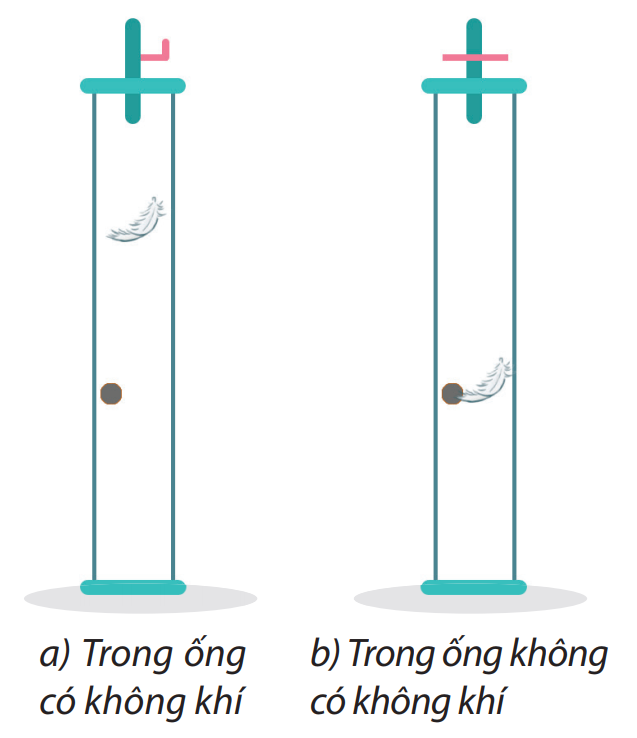
\includegraphics[scale=0.6]{figs/G10Y25B7-1}
		\captionof{figure}{Thí nghiệm về sự rơi tự do.}
	\end{center}
	\subsubsection{Nghiên cứu sự rơi tự do của các vật}
	\paragraph{Những đặc điểm của chuyển động rơi tự do}
	\begin{itemize}
		\item Phương của chuyển động rơi tự do là phương thẳng đứng (phương của dây dọi).
		\item Gia tốc của vật chuyển động rơi tự do chính là gia tốc rơi tự do.
		\item Chuyển động rơi tự do là chuyển động thẳng biến đổi đều.
	\end{itemize}	
	
	\paragraph{Gia tốc rơi tự do}
	Tại một nơi nhất định trên Trái Đất và ở gần mặt đất, mọi vật đều rơi tự do với cùng gia tốc.
	
	Gia tốc rơi tự do kí hiệu là $g$, giá trị của $g$ phụ thuộc vào vĩ độ địa lí và độ cao. Ở gần bề mặt Trái Đất người ta thường lấy giá trị của $g$ bằng $\SI{9.8}{\meter/\second^2}$.
	\paragraph{Các phương trình của sự rơi tự do}
	
	Phương trình vận tốc:
	
	\begin{equation*}
		v = v_0+g(t -t_0).
	\end{equation*}
	
	Phương trình tọa độ (gốc toạ độ tại vị trí ban đầu của vật, chiều dương cùng chiều chuyển động):
	
	\begin{equation*}
		y = y_0 +v_0(t-t_0)+ \dfrac{1}{2}g(t -t_0)^2.
	\end{equation*}
	
	Quãng đường đi được:
	
	\begin{equation*}
		d= s = v_0(t-t_0)+\dfrac{1}{2} g (t-t_0)^2
	\end{equation*}
	Liên hệ giữa vận tốc và quãng đường đi được:
	$$v^2-v^2_0=2gs$$
	
	Nếu ta chọn $t_{0}=0$ và vật được thả rơi không vận tốc đầu $v_0=0$ thì các công thức trên trở thành
	\begin{align*}
		v&=gt\\	
		y&=y_0+\dfrac{1}{2}gt^{2}\\
		d&=s=\dfrac{1}{2}gt^{2}\\
		v^2&=2gs
	\end{align*}
	\begin{luuy}
			Định nghĩa sự rơi tự do là chuyển động chỉ dưới tác dụng của trọng lực, tức là gia tốc của vật phải đúng bằng gia tốc rơi tự do $a=g$, chứ không quy định về vận tốc ban đầu của vật. \\
		Nói cách khác, thành phần chuyển động theo phương thẳng đứng của các vật chuyển động ném ngang, ném xiên đều được coi là chuyển động rơi tự do.
	\end{luuy}
	
	
	
\end{tomtat}
\subsection{VÍ DỤ MINH HỌA}
\begin{dang}{Nhận biết được đặc điểm của sự rơi tự do, gia tốc rơi tự do}
	\end{dang}
	\begin{vd}
		Câu nào sau đây nói về sự rơi là đúng?
		
		\choice
		{Khi không có sức cản, vật nặng rơi nhanh hơn vật nhẹ}
		{\True Ở cùng một nơi, mọi vật rơi tự do có cùng gia tốc}
		{Khi rơi tự do, vật nào ở độ cao hơn sẽ rơi với gia tốc lớn hơn}
		{Vận tốc của vật chạm đất, không phụ thuộc vào độ cao của vật khi rơi}
		\loigiai{
			Gia tốc rơi tự do $g$ không phụ thuộc khối lượng của vật, chỉ phụ thuộc vĩ độ địa lí, độ cao và cấu trúc địa chất nơi đo nó nên ở cùng một nơi, mọi vật rơi tự do có cùng gia tốc.
			
		}
	\end{vd}
	
	\begin{vd}
		Chuyển động của vật nào dưới đây có thể coi gần đúng như chuyển động rơi tự do?
		\choice
		{Một vận động viên nhảy dù đang rơi khi dù đã mở}
		{\True Một viên gạch rơi từ độ cao $\SI{3}{m}$ xuống đất}
		{Một chiếc thang máy đang chuyển động đi xuống}
		{Một chiếc lá đang rơi}
		\loigiai{
			Theo định nghĩa, sự rơi tự do (chuyển động rơi tự do) là sự rơi của các vật chỉ chịu tác dụng của trọng lực.
			
			Trong các trường hợp trên, vận động viên nhảy dù và chiếc lá đều chịu thêm tác động của lực cản không khí trong quá trình rơi; thang máy chịu thêm tác động của lực căng dây cáp. Các lực thêm vào này làm chuyển động của các vật này có gia tốc khác đáng kể với gia tốc rơi tự do. Do đó, các  chuyển động này không được xem là chuyển động rơi tự do. 
			
			Chuyển động của một viên gạch rơi từ độ cao $\SI{3}{m}$ xuống đất có thể xem gần đúng là chuyển động rơi tự do, vì trong khi rơi lực cản không khí không đáng kể so với trọng lực, nên gia tốc của viên gạch gần bằng gia tốc rơi tự do.
			
		}
	\end{vd}
	
	\begin{vd}
		Chọn phương án sai. Chuyển động rơi tự do không vận tốc đầu có
		\choice
		{phương thẳng đứng}
		{chiều từ trên xuống dưới}
		{\True là chuyển động thẳng chậm dần đều}
		{chỉ chịu tác dụng của trọng lực}
		\loigiai{
			Chuyển động rơi tự do không vận tốc đầu là chuyển động thẳng nhanh dần đều.
			
		}
	\end{vd}
\begin{dang}{Xác định vận tốc, quãng đường và thời gian của vật rơi tự do}
\end{dang}
\begin{vd}
	Một vật rơi tự do không vận tốc đầu, khi chạm đất thì vật đạt tốc độ $v = \SI{20}{m/s}$. Hỏi vật được thả rơi từ độ cao nào? Biết $g = \SI{10}{m/s}^2$.
	\loigiai{
		Ta có:
		$$v^2-v^2_0=2gh\Rightarrow h=\dfrac{v^2}{2g}=\dfrac{\left(\SI{20}{\meter/\second}\right)^2}{2\cdot\left(\SI{10}{\meter/\second^2}\right)}=\SI{20}{\meter}.$$
	}
\end{vd}

\begin{vd}
	Từ độ cao $\SI{120}{m}$ người ta thả một vật thẳng đứng xuống với vận tốc đầu $v_0 = \SI{10}{m/s}$. Cho biết gia tốc trọng trường $g = \SI{10}{m/s}^2$.
	\begin{enumerate}[label=\alph*.]
		\item Sau bao lâu vật chạm đất.
		\item Tính vận tốc của vật lúc vừa chạm đất. 
	\end{enumerate}
	\loigiai{
		\begin{enumerate}[label=\alph*.]
			\item Thời gian vật chạm đất được tính từ phương trình chuyển động
			
			$$s = v_0t + \dfrac{1}{2}gt^2 \quad\Leftrightarrow\quad 120 = 10t + 5t^2.$$
			Giải phương trình này, ta thu được hai nghiệm và chọn nghiệm dương
			$$\Rightarrow t = \SI{4}{s}\ (\text{nhận})\ \text{hoặc} \ t = -\SI{6}{s}\ (\text{loại}).$$
			
			\item Vận tốc của vật lúc vừa chạm đất
			$$v = v_0 + gt =\SI{10}{\meter/\second}+(\SI{10}{\meter/\second^{2}})\cdot\left(\SI{4}{\second}\right)= \SI{50}{m/s}.$$
		\end{enumerate}	
	\begin{luuy}
		Trong khi giải các phương trình chuyển động thẳng biến đổi đều để tìm thời gian, ta thường gặp trường hợp giải được hai nghiệm. Thông thường nghiệm dương sẽ được chọn vì đây là nghiệm ứng với thời điểm sau khi bắt đầu khảo sát hiện tượng. 
	\end{luuy}		
	}
\end{vd}

\begin{vd}
	Từ một đỉnh tháp cao $\SI{20}{\meter}$, người ta buông một vật. Sau $\SI{2}{\second}$ thì người ta lại buông vật thứ 2 ở tầng thấp hơn đỉnh tháp $\SI{5}{\meter}$. Chọn trục O$y$ thẳng đứng, gốc O ở đỉnh tháp, chiều dương hướng xuống, mốc thời gian lúc vật 1 bắt đầu rơi, $g=\SI{10}{\meter/\second^2}$.
	\begin{enumerate}[label=\alph*.]
		\item Lập phương trình chuyển động của hai vật.
		\item Hai vật có chạm đất cùng lúc không?
		\item Vận tốc lúc chạm đất của mỗi vật là bao nhiêu?
	\end{enumerate}
	\loigiai{
		\begin{enumerate}[label=\alph*.]
			\item 
			Vật thứ nhất xuất phát từ đỉnh tháp (là gốc tọa độ) và được buông (không vận tốc đầu) nên phương trình chuyển động có dạng 
			\begin{align*}
				y_1&=y_{01}+v_{01}t+\dfrac{1}{2}gt^2\\
				&=\SI{0}{\meter}+ \left(\SI{0}{\meter/\second}\right)\cdot t +\dfrac{1}{2}\cdot\left(\SI{10}{\meter/\second^{2}}\right)\cdot t^{2}\\
				&=5t^{2} \quad \left(\si{\meter}, \si{\second}\right).
			\end{align*}
			
			Phương trình chuyển động của vật 2 là:
			\begin{align*}
				y_{2}&=y_{02}+v_{02}t+\dfrac{1}{2}g(t-t_0)^2\\
				&=\SI{5}{\meter}+(\SI{0}{\meter/\second})\cdot (t-\SI{2}{\second})+\dfrac{1}{2}\cdot(\SI{10}{\meter/\second^{2}})\cdot (t-\SI{2}{\second})^{2}\\
				&=5t^2-20t+25\quad \left(\si{\meter}, \si{\second}\right)\qquad \textrm{với }t>2.
			\end{align*}
			\item 
			Thời điểm vật 1 chạm đất:
			\begin{equation*}
				y_1=5t^2=\SI{20}{\meter}\Rightarrow t_1=\SI{2}{\second}.
			\end{equation*}
			
			Thời điểm vật 2 chạm đất:
			\begin{equation*}
				\begin{gathered}
					y_{2}=5t^2-20t+25=\SI{20}{\meter}\\ \quad\Rightarrow\quad t_2=\SI{3.73}{\second}\textrm{ (nhận) hoặc } t_2=\SI{0.27}{\second}\textrm{ (loại)}.
				\end{gathered}
			\end{equation*}
			Ở đây nghiệm $\SI{0.27}{\second}$ bị loại vì đây là thời điểm trước khi vật 2 được thả, không phù hợp với hiện tượng được mô tả trong đề. 
			
			Vậy hai vật không chạm đất cùng lúc.
			\item Vận tốc lúc chạm đất của mỗi vật là:
			\begin{align*}
				v_1&=gt_1=\left(\SI{10}{\meter/\second^{2}}\right)\cdot\left(\SI{2}{\second}\right)=\SI{20}{\meter/\second},\\
				v_2&=g(t_2-t_0)=\left(\SI{10}{\meter/\second^{2}}\right)\cdot(\SI{3.73}{\second}-\SI{2}{\second})=\SI{17.3}{\meter/\second}.
			\end{align*}
		\end{enumerate}
	}
\end{vd}
\begin{dang}{Xác định quãng đường vật đi được \\trong giây thứ $n$, hoặc trong $n$ giây cuối}
	Quãng đường rơi được trong $n$ giây kể từ thời điểm được thả rơi: 
	$$s_n=\dfrac{1}{2}\cdot g \cdot n^2$$
	Quãng đường rơi được trong giây thứ $n$ là quãng đường vật đi được từ thời điểm $\left(n-1\right)$ giây đến thời điểm $n$ giây
	$$\Delta s_n=s_n-s_{n-1}=\dfrac{1}{2}\cdot g\cdot n^2 -\dfrac{1}{2}\cdot g \left(n-1\right)^2$$
	\end{dang}
	\begin{vd}
		Một vật rơi tự do không vận tốc đầu tại nơi có gia tốc trọng trường $g$. Trong giây thứ 3, quãng đường rơi được là $\SI{24,5}{m}$ và tốc độ của vật khi vừa chạm đất là $\SI{39,2}{m/s}$. Tính gia tốc trọng trường $g$ tại nơi thả vật và độ cao ban đầu của vật.
		\loigiai{
			Quãng đường vật rơi trong 3 giây: 
			$$s_1 = \dfrac{1}{2}gt^2_1 =4,5g.$$	
			
			Quãng đường vật rơi trong 2 giây đầu: 
			$$s_2 = \dfrac{1}{2}gt^2_2 =2g.$$	
			
			Quãng đường vật rơi trong giây thứ 3: 
			$$\Delta s = s_1 - s_2 \quad\Leftrightarrow\quad \SI{24,5}{m} = 4,5g - 2g \quad\Rightarrow g = \SI{9,8}{m/s^2}.$$
			
			Độ cao lúc thả vật: 
			$$s =\dfrac{v^2}{2g} =\SI{80}{m}.$$
			
		}
	\end{vd}
	
	\begin{vd}
		Một vật rơi tự do từ độ cao $h$. Biết rằng trong $\SI{2}{s}$ cuối cùng vật rơi được quãng đường bằng quãng đường đi trong $\SI{5}{s}$ đầu tiên, $g = \SI{10}{m/s^2}$.
		\begin{enumerate}[label=\alph*.]
			\item Tìm độ cao lúc thả vật và thời gian vật rơi.
			
			\item Tìm tốc độ của vật lúc vừa chạm đất.
			
		\end{enumerate}
		\loigiai{
			\begin{enumerate}[label=\alph*.]
				\item Chọn chiều dương hướng xuống, gốc toạ độ tại vị trí vật bắt đầu rơi, gốc thời gian lúc vật rơi. 
				
				Quãng đường vật rơi trong $t$ giây: 
				$$s = \dfrac{1}{2}gt^2.$$
				
				Quãng đường vật rơi trong ($t - 2$) giây: 
				$$s_1 =\dfrac{1}{2}g(t-2)^2.$$
				
				Quãng đường vật rơi trong 5 giây đầu tiên: 
				$$s_5 = \dfrac{1}{2}g t_5^2.$$
				
				Quãng đường vật rơi trong 2 giây cuối: 
				$$s_2 = s - s_1 = s_5 \quad\Leftrightarrow\quad  \dfrac{1}{2}gt^2 - \dfrac{1}{2}g(t-2)^2 = \dfrac{1}{2}g t_5^2 \quad\Rightarrow\quad t = \SI{7,25}{s}.$$
				
				Độ cao lúc thả vật:
				$$s = \dfrac{1}{2}gt^2= \SI{262,81}{m}.$$
				\item  Tốc độ của vật lúc vừa chạm đất:
				
				$$v = gt = \SI{72,5}{m/s}.$$
			\end{enumerate}
		}
	\end{vd}
\begin{dang}{Khảo sát chuyển động của vật bị ném theo phương thẳng đứng}
\end{dang}
\begin{vd}
	Một vật được ném lên thẳng đứng từ mặt đất, bỏ qua lực cản của không khí. Tính độ cao cực đại mà vật đạt được biết vận tốc ban đầu của vật là $\SI{20}{m/s}$, lấy $g = \SI{10}{m/s^2}$.
	\loigiai{
		Chọn chiều dương hướng lên, chuyển động của vật là chuyển động thẳng chậm dần đều với gia tốc $a = -g = -\SI{10}{m/s^2}$ và vận tốc ban đầu $v_0=\SI{20}{m/s}.$
		
		Độ cao cực đại bằng quãng đường mà vật đi được đến khi dừng lại ($v=0$)
		$$v^2 - v_0^2=2as \Rightarrow s= h_\text{max}= \SI{20}{m}.$$
	}
\end{vd}

\begin{vd}
	Một vật được ném lên theo phương thẳng đứng từ mặt đất. Sau $\SI{4}{s}$ vật lại rơi xuống mặt đất. Cho $g = \SI{10}{m/s^2}$. Tính
	\begin{enumerate}[label=\alph*)]
		\item Vận tốc ban đầu của vật.
		
		\item Độ cao tối đa mà vật lên tới.
		
		\item Vận tốc của vật ở độ cao bằng $\dfrac{3}{4}$ độ cao tối đa.
	\end{enumerate}
	\loigiai{
		\begin{enumerate}[label=\alph*)]
			\item Chọn gốc toạ độ tại vị trí ném, chiều dương hướng lên, gốc thời gian lúc ném vật. Phương trình chuyển động của vật có dạng 
			$$y =v_0t - \dfrac{1}{2}gt^2.$$
			Vật chạm đất khi $y=0$, do đó 
			\begin{align*}
				y&= v_0t -\dfrac{1}{2}gt^2=0\\
				\Rightarrow\quad v_0 &=\dfrac{gt}{2}=\dfrac{
					\SI{10}{\meter/\second^2}\cdot
					\SI{4}{\second}
				}{2} =\SI{20}{\meter/\second}.
			\end{align*}
			\item Khi vật lên đến độ cao tối đa, vận tốc của vật triệt tiêu $v=0$. Độ cao của vật khi đó cũng chính là quãng đường vật đã đi được 
			\begin{align}
				v^2-v_0^2 =-2gh \quad\Rightarrow\quad h =\dfrac{v^2 -v_0^2}{-2g}=\dfrac{(\SI{0}{\meter/\second})^2-(\SI{20}{\meter/\second})^2}{-2\cdot\SI{10}{\meter/\second^{2}}}=\SI{20}{\meter}.
			\end{align}
			\item Sử dụng công thức liên hệ 
			$v_1^2-v_0^2 =2as=-2gh_1,$ 
			trong đó độ cao $h_1=\dfrac{3}{4}h=\SI{15}{m}$,
			ta suy ra vận tốc của vật khi đó 
			\begin{eqnarray*}
				v_1^2&=&v_0^2 -2gh_1=(\SI{20}{\meter/\second})^2-2\cdot\SI{10}{\meter/\second^{2}}\cdot\SI{15}{\meter}=\SI{100}{\meter^2/\second^2}\\
				\Rightarrow\quad v_1&=&\pm \SI{10}{\meter/\second}.
			\end{eqnarray*}
			Giá trị dương của vận tốc ứng với thời điểm vật đang đi lên, giá trị âm ứng với thời điểm vật đang đi xuống. 
		\end{enumerate}
	}
\end{vd}

\begin{vd}
	Một viên bi A được thả rơi từ độ cao $\SI{30}{\meter}$. Cùng lúc đó, một viên bi B được bắn theo phương thẳng đứng từ dưới đất lên với vận tốc ban đầu $\SI{25}{\meter/\second}$ tới va chạm vào bi A. Chọn trục O$y$ thẳng đứng, gốc O ở mặt đất, chiều dương hướng lên, gốc thời gian lúc 2 viên bi bắt đầu chuyển động, $g=\SI{10}{\meter/\second^2}$. Bỏ qua sức cản không khí.
	\begin{enumerate}[label=\alph*.]
		\item Lập phương trình chuyển động của mỗi viên bi.
		\item Tính thời điểm và tọa độ 2 viên bi gặp nhau.
		\item  Vận tốc mỗi viên bi khi gặp nhau.
	\end{enumerate}
	\loigiai{
		\begin{enumerate}[label=\alph*.]
			\item 
			Phương trình chuyển động của viên bi A là
			\begin{align*}
				y_{\text{A}}&=y_{0\text{A}}+v_{0\text{A}}t+\dfrac{1}{2}gt^2\\
				&=30+0\times t-\dfrac{1}{2}\times 10\times t^{2}\\
				&=30-5t^2 \textrm{ (m, s)}.
			\end{align*}
			
			Phương trình chuyển động của viên bi B là
			\begin{align*}
				y_{\text{B}}&=y_{0\text{B}}+v_{0\text{B}}t+\dfrac{1}{2}gt^2\\
				&=0+25t-\dfrac{1}{2}\times10\times t^{2}\\
				&=25t-5t^2\textrm{ (m, s)}.
			\end{align*}
			\item 
			Hai viên bi gặp nhau khi chúng có cùng tọa độ
			\begin{equation*}
				y_{\text{A}}=y_{\text{B}}\Rightarrow 30-5t^2=25t-5t^2 \Rightarrow t=\SI{1.2}{\second}.
			\end{equation*}
			
			Khi đó hai viên bi đang ở tọa độ 
			\begin{equation*}
				y_{\text{A}}=y_{\text{B}}=30-5t^2=\SI{22.8}{\meter}.
			\end{equation*}
			\item  Vận tốc của mỗi viên bi khi gặp nhau là:
			\begin{equation*}
				\left\{\begin{array}{ll}{v_{\text{A}}=-gt=\SI{-12}{\meter/\second}}&\\{v_{\text{B}}=v_0-gt=\SI{13}{\meter/\second}.}&\end{array}\right.
			\end{equation*}
			Vận tốc của bi 1 âm cho thấy bi 1 đang chuyển động hướng xuống (ngược chiều dương), còn bi 2 có vận tốc dương cho tương ứng đang chuyển động hướng lên (cùng chiều dương).
		\end{enumerate}
	}
\end{vd}
\subsection{TRẮC NGHIỆM NHIỀU PHƯƠNG ÁN LỰA CHỌN}
\setcounter{ex}{0}
\Opensolutionfile{ans}[ans/G10Y25B7-TN]
\begin{ex}
	Câu nào sau đây là đúng khi nói về sự rơi?
	\choice
	{Khi không có sức cản vật năng rơi nhanh hơn vật nhẹ}
	{\True Ở cùng một nơi, mọi vật rơi tự do có cùng gia tốc}
	{Khi rơi tự do, vật nào ở độ cao lớn hơn sẽ rơi với gia tốc lớn hơn}
	{Vận tốc của vật chạm đất không phụ thuộc vào độ cao của vật khi rơi}
	\loigiai{	
		Gia tốc rơi tự do không phụ thuộc vào khối lượng của vật, chỉ phụ thuộc vào vĩ độ địa lý, độ cao và cấu trúc địa chất nơi đó nên ở cùng một nơi, mọi vật rơi tự do có cùng gia tốc.
	}
\end{ex}

\begin{ex}
	Thí nghiệm của Galilei ở tháp nghiêng Pisa và ống Newton chứng tỏ
	\choice
	{mọi vật đều rơi theo phương thẳng đứng}
	{rơi tự do là chuyển đông nhanh dần đều}
	{\True các vật nặng, nhẹ đều rơi tự do như nhau}
	{vật nặng rơi nhanh hơn vật nhẹ}
	\loigiai{
	}
\end{ex}

\begin{ex}
	Vật nào được xem là rơi tự do?
	\choice
	{Viên đạn đang bay trong không trung}
	{Phi công đang nhảy dù}
	{\True Qủa táo rơi từ trên cây xuống}
	{Máy bay đang bay gặp tai nạn và lao xuống}
	\loigiai{
	}
\end{ex}

\begin{ex}
	Gia tốc rơi tự do phụ thuộc vào những yếu tố nào?
	\choice
	{Khối lượng và kích thước vật rơi}
	{\True Độ cao và vĩ độ địa lý}
	{Vận tốc đầu và thời gian rơi}
	{Áp suất và nhiệt độ môi trường}
	\loigiai{
	}
\end{ex}

\begin{ex}
	Tại một nơi có gia tốc trọng trường $g$, một vật có khối lượng $m$ rơi tự do từ độ cao $h$ xuống mặt đất. Ngay trước khi chạm đất vật đạt tốc độ
	\choice
	{$v=mgh$}
	{$v=2\sqrt{gh}$}
	{\True $v=\sqrt{2gh}$}
	{$v=\sqrt{gh}$}
	\loigiai{
	}
\end{ex}

\begin{ex}
	Một giọt nước rơi tự do từ độ cao $\SI{45}{\meter}$ xuống. Sau bao lâu nó rơi tới mặt đất? Cho $g=\SI{10}{\meter/\second^2}$.
	\choice
	{$\SI{2.1}{\second}$}
	{\True $\SI{3}{\second}$}
	{$\SI{4.5}{\second}$}
	{$\SI{9}{\second}$}
	\loigiai{
		Thời gian rơi:
		$$t=\sqrt{\dfrac{2h}{g}}=\SI{3}{\second}.$$
	}
\end{ex}

\begin{ex}
	Người ta thả một vật rơi tự do, sau $\SI{5}{\second}$ vật chạm đất, $g=\SI{9.8}{\meter/\second^2}$. Độ cao thả vật là
	\choice
	{\True $\SI{122.5}{\meter}$}
	{$\SI{61.25}{\meter}$}
	{$\SI{254}{\meter}$}
	{$\SI{183,75}{\meter}$}
	\loigiai{	
		Độ cao lúc thả vật là:
		$h=s=\dfrac{1}{2}gt^2=\dfrac{1}{2}\cdot\SI{9.8}{\meter/\second^2}\cdot(\SI{5}{\second})^2=\SI{122.5}{\meter}.$
	}
\end{ex}

\begin{ex}
	Thả hai vật rơi tự do đồng thời từ hai độ cao $h_1$ và $h_2$. Biết rằng thời gian chạm đất của vật thứ nhất bằng 2 lần của vật thứ hai. Tỉ số $\dfrac{h_1}{h_2}$ là
	\choice
	{\True $\dfrac{h_1}{h_2}=4$}
	{$\dfrac{h_1}{h_2}=\dfrac{1}{2}$}
	{$\dfrac{h_1}{h_2}=2$}
	{$\dfrac{h_1}{h_2}=\dfrac{1}{4}$}
	\loigiai{	
		Tỉ số $\dfrac{h_1}{h_2}$ có thể được suy ra từ việc lập tỉ số độ cao của hai vật: $$\dfrac{h_1}{h_2}=\dfrac{\dfrac{1}{2}gt_1^2}{\dfrac{1}{2}gt_2^2}=\dfrac{t_1^2}{t_2^2}=\left( \dfrac{t_1}{t_2}\right)^2=4.$$
	}
\end{ex}

\begin{ex}
	Một hòn đá thả rơi tự do từ đỉnh toà nhà $25$ tầng nó chạm đất trong thời gian $5\ \text{s}$. Lấy $g=10\ \text{m/s}^2$. Trong giây đầu tiên hòn đá đã đi qua số tầng của toà nhà là
	\choice
	{\True $1$}
	{$2$}
	{$3$}
	{$5$}
	\loigiai{	
		Gọi chiều cao mỗi tầng nhà là $h$. 
		
		Suy ra $25h=g\dfrac{5^2}{2}\Rightarrow h=5\ \text{m}$.
		
		Gọi $n$ là số tầng trong giây đầu hòn đá rơi được.
		
		Suy ra $n\cdot 5=g\cdot \dfrac{1^2}{2}\Rightarrow n=1$.
	}
\end{ex}

\begin{ex}
	Từ đỉnh tháp hai vật A và B được thả rơi tự do. Biết B được thả rơi sau A $1\ \text{s}$. Lấy $g=10\ \text{m/s}^2$. Khoảng cách giữa A và B tại thời điểm sau khi B rơi được $2\ \text{s}$ là
	\choice
	{$5\ \text{m}$}
	{$10\ \text{m}$}
	{$20\ \text{m}$}
	{\True $25\ \text{m}$}
	\loigiai{	
		Tại thời điểm sau khi B rơi được $2\ \text{s}$, A đã rơi được $3\ \text{s}$
		
		Suy ra, khoảng cách giữa A và B là:
		
		$\Delta h=g\cdot\dfrac{t_1^2}{2}-g\cdot\dfrac{t_2^2}{2}=\dfrac{10}{2}\cdot \left( 3^2-2^2\right)=25\ \text{m}$.
	}
\end{ex}

\begin{ex}
	Một người thả vật rơi tự do, vật chạm đất có $v=\SI{36}{\meter/\second}$, $g=\SI{10}{\meter/\second^2}$. Độ cao của vật sau khi thả được $\SI{3}{\second}$ là
	\choice
	{$\SI{64.8}{\meter}$}
	{\True $\SI{19.8}{\meter}$}
	{$\SI{86.4}{\meter}$}
	{$\SI{45.0}{\meter}$}
	\loigiai{	
		Độ cao nơi thả vật:
		$$v=\sqrt{2gh}\Rightarrow h = \SI{64.8}{\meter}.$$
		Quãng đường vật rơi $\SI{3}{\second}$ đầu tiên là:
		$$s_3=\dfrac{1}{2}gt^2=\dfrac{1}{2}\cdot\SI{10}{\meter/\second^2}\cdot(\SI{3}{\second})^2=\SI{45}{\meter}.$$
		Độ cao của vật lúc này:
		$$h=s-s_3=\SI{64.8}{\meter}-\SI{45}{\meter}=\SI{19.8}{\meter}.$$
	}
\end{ex}

\begin{ex}
	Các giọt nước mưa đang rơi từ mái nhà xuống sau những khoảng thời gian bằng nhau. Khi giọt thứ nhất chạm đất thì giọt thứ năm bắt đầu rơi, lúc đó khoảng cách giữa giọt thứ nhất và giọt thứ hai là $\SI{14}{\meter}$. Lấy $g=\SI{10}{\meter/\second^2}$. Độ cao mái nhà là
	\choice
	{\True $\SI{32}{\meter}$}
	{$\SI{9}{\meter}$}
	{$\SI{56}{\meter}$}
	{$\SI{16}{\meter}$}
	\loigiai{	
		Gọi $\Delta t$ khoảng thời gian bằng nhau các giọt nước mưa đang rơi từ mái nhà xuống.
		
		Quãng đường giọt thứ nhất rơi cho đến khi chạm đất là:
		$$s_1=\dfrac{1}{2}g(4\Delta t)^2.$$
		Quãng đường giọt thứ hai rơi cho đến khi giọt thứ nhất chạm đất là:
		$$s_2=\dfrac{1}{2}g(3\Delta t)^2.$$
		Theo đề bài ta có:
		$$\Delta s= s_1-s_2=\dfrac{7}{2}g(\Delta t)^2=\SI{14}{\meter}\Rightarrow \Delta t=\dfrac{\sqrt{10}}{5}\,\text{s}.$$
		Độ cao mái nhà là:
		$$h=s_1=\dfrac{1}{2}g(4\Delta t)^2=\SI{32}{\meter}.$$
	}
\end{ex}

\begin{ex}
	Thả một hòn đá từ mép một vách núi dựng đứng xuống vực sâu. Sau $\SI{3.96}{\second}$ từ lúc thả thì nghe thấy tiếng hòn đá chạm đáy vực sâu. Biết $g=\SI{9.8}{\meter/\second^2}$ và tốc độ truyền âm trong không khí là $\SI{330}{\meter/\second}$. Chiều cao vách đá là
	\choice
	{$\SI{76}{\meter}$}
	{$\SI{58}{\meter}$}
	{\True $\SI{69}{\meter}$}
	{$\SI{82}{\meter}$}
	\loigiai{
		$$t=\dfrac{h}{v_a}+\sqrt{\dfrac{2h}{g}}\Rightarrow h\approx\SI{69}{\meter}.$$
	}
\end{ex}

\begin{ex}
	Một vật rơi tự do từ độ cao $250\ \text{m}$. Tỉ số quãng đường vật rơi được trong $2\ \text{s}$ đầu, $2\ \text{s}$ sau và $2\ \text{s}$ cuối cùng là
	\choice
	{$1:4:9$}
	{$1:2:4$}
	{\True $1:3:5$}
	{$1:2:3$}
	\loigiai{	
		Rơi tự do là chuyển động nhanh dần đều với $v_0=0$  nên khi thời gian chuyển động trên các đoạn đường liên tiếp bằng nhau (cùng bằng $2\ \text{s}$) thì $\Delta s_1:\Delta s_2:\Delta s_3=1:3:5$.
	}
\end{ex}

\begin{ex}
	Quãng đường vật rơi trong giây thứ $n$ là $h$. Quãng đường mà nó rơi trong giây tiếp theo là
	\choice
	{$h$}
	{$\left(h+\dfrac{g}{2}\right)$}
	{$(h-g)$}
	{\True $(h+g)$}
	\loigiai{	
		Quãng đường vật rơi được trong giây thứ $n$ bằng quãng đường vật rơi được từ ban đầu cho đến giây $n$ trừ cho quãng đường vật rơi được từ ban đầu cho đến giây $n-1$: $$h=\dfrac{g}{2}(2n-1)$$
		
		Quãng đường vật rơi được trong giây thứ $n+1$ bằng quãng đường vật rơi được từ ban đầu cho đến giây $n+1$ trừ cho quãng đường vật rơi được từ ban đầu cho đến giây $n$:
		$$h'=\dfrac{1}{2}g(n+1)^2-\dfrac{1}{2}gn^2 = \dfrac{g}{2}(2n+1)$$
		
		Vậy $h'=h+g$.
	}
\end{ex}
\Closesolutionfile{ans}
\subsection{TRẮC NGHIỆM ĐÚNG SAI}
\setcounter{ex}{0}
\Opensolutionfile{ans}[ans/G10Y25B7-TF]

\Closesolutionfile{ans}
\subsection{TRẢ LỜI NGẮN}
\setcounter{ex}{0}
\Opensolutionfile{ans}[ans/G10Y25B7-SA]

\Closesolutionfile{ans}
\subsection{TỰ LUẬN}
\setcounter{ex}{0}
\Opensolutionfile{ans}[ans/G10Y25B7-TL]
\begin{ex}
	Sự rơi tự do là gì? Nêu các đặc điểm của sự rơi tự do.
	\loigiai{
		Sự rơi tự do là sự rơi của các vật chỉ dưới tác dụng của trọng lực.
		
		Các đặc điểm của sự rơi tự do:
		\begin{itemize}
			\item Phương của chuyển động rơi tự do là phương thẳng đứng;
			\item Chiều của chuyển động rơi tự do là chiều từ trên xuống dưới;
			\item Chuyển động rơi tự do là chuyển động thẳng nhanh dần đều.
		\end{itemize}
	}
\end{ex}

\begin{ex}
	Một vật nặng rơi không vận tốc đầu từ độ cao $\SI{20}{m}$ xuống đất. Tính thời gian rơi và vận tốc của vật khi chạm đất. Lấy $g=\SI{10}{m/s^2}$.
	\loigiai{
		Thời gian chạm đất:
		$$t=\sqrt{\dfrac{2h}{g}}=\SI{2}{\second}.$$
		
		Vận tốc của vật khi chạm đất:
		$$v=gt = \SI{20}{m/s}.$$
	}
\end{ex}

\begin{ex}
	Thả một hòn đá từ độ cao $h$ xuống đất, hòn đá rơi trong $\SI{1}{s}$. Nếu thả hòn đá đó từ $h’ = 4h$ thì thời gian rơi là bao nhiêu?
	\loigiai{
		Ta có:
		$$h = \dfrac{1}{2} gt^2 \Rightarrow t =\sqrt{\dfrac{2h}{g}} = \SI{1}{s}.$$
		
		Lại có:
		$$h' = \dfrac{1}{2}gt_1^2 \Rightarrow t_1 = \sqrt{\dfrac{2h'}{g}}=2\sqrt{\dfrac{2h}{g}} =\SI{2}{s}.$$
	}
\end{ex}

\begin{ex}
	Một vật được thả rơi không vận tốc đầu khi vừa chạm đất có tốc độ $v=\SI{70}{m/s}$, $g = \SI{10}{m/s^2}$.
	\begin{enumerate}[label=\alph*)]
		\item Xác định quãng đường rơi của vật.
		\item Tính thời gian rơi của vật.
	\end{enumerate}
	\loigiai{
		\begin{enumerate}[label=\alph*)]
			\item Quãng đường rơi của vật
			$$v^2 - v^2_0 = 2gS \Rightarrow S = \dfrac{v^2-v^2_0}{2g} = \SI{245}{m}.$$
			
			\item Thời gian rơi của vật
			$$v = gt \Rightarrow t = \dfrac{v}{g} =\SI{7}{s}.$$
		\end{enumerate}
	}
\end{ex}

\begin{ex}
	Từ độ cao $\SI{120}{m}$ người ta ném một vật thẳng đứng xuống với tốc độ ban đầu $v_0 = \SI{10}{m/s}$, $g = \SI{10}{m/s^2}$.
	\begin{enumerate}[label=\alph*)]
		\item Sau bao lâu vật chạm đất?
		\item Tính vận tốc của vật lúc vừa chạm đất.
	\end{enumerate}
	\loigiai{
		\begin{enumerate}[label=\alph*)]
			\item Thời gian vật chạm đất
			$$s = v_0t + \dfrac{1}{2}gt^2 \Rightarrow t =\SI{4}{s}.$$
			
			\item Vận tốc của vật lúc vừa chạm đất
			$$v = v_0 +gt = \SI{50}{m/s}.$$
		\end{enumerate}
	}
\end{ex}

\begin{ex}
	Một người thả một hòn bi từ trên cao xuống đất và đo được thời gian rơi là $\SI{3,1}{s}$. Bỏ qua sức cản không khí. Lấy $g=\SI{9,8}{m/s^2}$.
	\begin{enumerate}[label=\alph*)]
		\item Tính độ cao của nơi thả hòn bi so với mặt đất và vận tốc lúc chạm đất.
		\item Tính quãng đường rơi được trong $\SI{0,5}{s}$ cuối trước khi chạm đất.
	\end{enumerate}
	\loigiai{	
		\begin{enumerate}[label=\alph*)]
			\item Độ cao của nơi thả hòn bi so với mặt đất 
			$$h = \dfrac{1}{2}gt^2 = \SI{47,089}{m}.$$
			
			Vận tốc lúc chạm đất
			$$ v = gt = \SI{30,38}{m/s}.$$
			
			\item Quãng đường rơi được trong $\SI{0,5}{s}$ cuối trước khi chạm đất
			$$h' = \dfrac{1}{2} g(t - \SI{0.5}{s})^2 = \SI{33,124}{m}.$$
		\end{enumerate}
	}
\end{ex}

\begin{ex}
	Hai viên bi sắt được thả rơi cùng độ cao cách nhau một khoảng thời gian $\SI{0,5}{\second}$. Lấy $g = \SI{10}{\meter/\second^2}$. Tìm khoảng cách giữa hai viên bi sau khi viên thứ nhất rơi được $\SI{1,5}{\second}$.
	\loigiai{	
		Chọn gốc thời gian là lúc thả viên bi 1. Viên bi 2 được thả sau $\SI{0,5}{\second}$ nên:
		$$t_2=t_1-\SI{0,5}{\second}.$$
		Quãng đường viên bi 1 đi được:
		$$s_1=\dfrac{1}{2}gt_1^2.$$
		Quãng đường viên bi 2 đi được:
		$$s_2=\dfrac{1}{2}g(t_1-\SI{0.5}{s})^2.$$
		Lấy $s_1-s_2=\dfrac{1}{2}gt_1^2-\dfrac{1}{2}g(t_1-\SI{0.5}{s})^2=\SI{6,25}{\meter}$.
	}
\end{ex}

\begin{ex}
	\begin{enumerate}[label=\alph*)]
		\item Người ta ném một vật nhỏ từ mặt đất lên cao theo phương thẳng đứng với tốc độ đầu $\SI{8}{\meter/\second}$. Lấy $g=\SI{10}{\meter/\second^2}$. Xác định độ cao cực đại mà vật đạt được.
		\item Một người thợ xây ném một viên gạch theo phương thẳng đứng cho một người khác ở trên tầng cao $\SI{4}{\meter}$. Người này chỉ việc giơ tay ngang ra là bắt được viên gạch. Lấy $g=\SI{10}{\meter/\second^2}$. Để cho viên gạch lúc người kia bắt được bằng không thì vận tốc lúc ném là bao nhiêu?
	\end{enumerate}
	\loigiai{
		\begin{enumerate}[label=\alph*)]
			\item Khi vật đạt độ cao cực đại thì vận tốc của vật bằng 0.\\
			Độ cao cực đại mà vật đạt được:
			$$h_\text{max}=\dfrac{0-v^2_0}{-2g}=\SI{3.2}{\meter}.$$
			\item Để khi đến tay người kia tốc độ của viên gạch bằng 0 thì tốc độ ban đầu của viên gạch là
			$$0-v^2_0=-2gh\Rightarrow v_0=\sqrt{2gh}\approx\SI{8.94}{\meter/\second}.$$
		\end{enumerate}
	}
\end{ex}

\begin{ex}
	Một hòn đá rơi tự do từ cửa sổ một toà nhà cao tầng. Sau đó $\SI{1}{s}$ tại ban công phía dưới cách cửa sổ trên của toà nhà $\SI{20}{m}$ có một hòn đá khác cũng rơi tự do. Biết cả hai hòn đá cùng chạm đất đồng thời. Lấy $g=10\ \text{m/s}^2$. Tìm chiều cao của cửa sổ toà nhà trên so với đất.	
	\loigiai{	
		Ta có: $h=g\cdot \dfrac{t^2}{2}; \ h-\SI{20}{m}=g\cdot \dfrac{\left(t-\SI{1}{s} \right)^2 }{2}$.
		
		$\Rightarrow t=\SI{2.5}{s}; \ h=\SI{31.25}{m}$.  
	}
\end{ex}

\begin{ex}
	Căn cứ vào số liệu cho trong bảng để :
	\begin{center}
		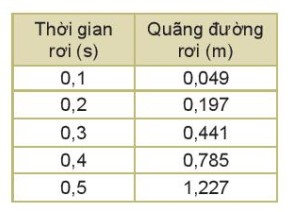
\includegraphics[scale=1]{figs/G10Y25B7-2}
	\end{center}
	\begin{enumerate}[label=\alph*)]
		\item Chứng tỏ chuyển động rơi tự do là nhanh dần đều. 
		\item Tính gia tốc của chuyển động rơi tự do.
	\end{enumerate}
	\loigiai{	
		\begin{enumerate}[label=\alph*)]
			\item 
			+ Từ giây thứ $\SI{0,1}{s}$ đến $\SI{0,2}{s}$, vật rơi được
			
			$$\Delta S_1 = S_2 -  S_1=0,197 - 0,049 = \SI{0,148}{m}.$$
			
			+ Từ giây thứ $\SI{0,2}{s}$ đến $\SI{0,3}{s}$, vật rơi được một khoảng là: 
			
			$$\Delta S_2 = S_3 -  S_2= 0,441 - 0,197= \SI{0,244}{m}.$$
			
			+ Từ giây thứ $\SI{0,3}{s}$ đến $\SI{0,4}{s}$, vật rơi được một khoảng là :
			
			$$\Delta S_3= S_4 - S_3= 0,785 - 0,441= \SI{0,344}{m}.$$
			
			Như vậy, sau cùng $\SI{0,1}{s}$ như nhau nhưng vật rơi được những khoảng khác nhau, càng về sau thì rơi càng nhanh hơn. 
			
			\item Dựa vào công thức:
			
			$$S = \dfrac{1}{2}gt^2 \Rightarrow g = \dfrac{2S}{t^2}.$$
			
			Ta có
			
			+ Gia tốc tại $t_1$ $\SI{0,1}{s}$ là: 
			
			$$g_1 = \dfrac{2 S_1}{t_1^2}= \SI{9,8}{m/s^2}.$$
			
			+ Gia tốc tại $t_2$ $\SI{0,2}{s}$ là: 
			
			$$g_2 = \dfrac{2 S_2}{t_2^2}=\SI{9,85}{m/s^2}.$$
			
			+ Gia tốc tại $t_3$ $\SI{0,3}{s}$ là: 
			
			$$g_3 = \dfrac{2 S_3}{t_3^2}=\SI{9,8}{m/s^2}.$$
			
			+ Gia tốc tại $t_4$ $\SI{0,4}{s}$ là: 
			$$g_4 = \dfrac{2S_4}{t_4^2}=\SI{9,8125}{m/s^2}.$$
			
			
		\end{enumerate}
	}
\end{ex}

\begin{ex}
	Từ tầng 9 của một tòa nhà, Minh thả rơi viên bi A. Sau $\SI{1}{s}$, Thắng thả rơi viên bi B ở tầng thấp hơn $\SI{10}{m}$. Hai viên bi sẽ gặp nhau lúc nào (tính từ khi viên bi A rơi), cho biết $g =\SI{9,8}{m/s^2}$.
	\loigiai{		Chọn trục gốc toạ độ tại vị trí thả viên bi A, chiều dương hướng xuống, gốc thời gian lúc thả bi A.
		
		Phương trình chuyển động của hai viên bi có dạng
		\begin{align*}
			y_1 &= y_{01} + \dfrac{1}{2}gt^2 =\dfrac{1}{2}gt^2,\\
			y_2 &= y_{02} + \dfrac{1}{2}g(t-t_0)^2 =\SI{10}{m}+\dfrac{1}{2}g(t-\SI{1}{s})^2.
		\end{align*}
		
		Khi 2 viên bi gặp nhau, tọa độ của chúng trùng nhau 
		\begin{align*}
			y_1=y_2 \quad\Leftrightarrow\quad \dfrac{1}{2}gt^2 =\SI{10}{m} + \dfrac{1}{2}g(t-\SI{1}{s})^2 \quad\Rightarrow\quad t =\SI{1.5}{\second}.
		\end{align*}
	}
\end{ex}

\begin{ex}
	Thả rơi tự do một vật từ độ cao $\SI{180}{m}$ so với mặt đất, đồng thời ném một vật từ mặt đất lên với vận tốc $\SI{80}{m/s}$, lấy $g = \SI{10}{m/s^2}$. Xác định độ cao so với mặt đất mà hai vật gặp nhau.
	\loigiai{	Chọn gốc tọa độ tại vị trí thả, gốc thời gian khi bắt đầu thả vật. Trục tọa độ có chiều dương hướng xuống.
		
		Phương trình chuyển động của vật rơi xuống
		$$y_1 =\dfrac{1}{2}gt^2.$$
		Phương trình chuyển động của vật được ném lên
		$$y_2 =\SI{180}{m} - \SI{80}{m/s}\cdot t + \dfrac{1}{2}gt^2.$$
		Khi hai vật gặp nhau, tọa độ của chúng bằng nhau
		$$y_1=y_2 \quad
		\Rightarrow\quad t =\SI{2.25}{\second}.$$
		Độ cao nơi gặp nhau:
		$$h = \SI{180}{m} - \dfrac{1}{2}gt^2 = \SI{154.69}{\meter}.$$		
		
	}
\end{ex}

\begin{ex}
	Ném một hòn sỏi từ mặt đất lên cao theo phương thẳng đứng với vận tốc $\SI{4}{\meter/\second}$. Lấy $g = \SI{10}{\meter/\second^2}$. Trong suốt quá trình từ lúc ném cho đến khi chạm đất, khoảng thời gian giữa hai thời điểm mà vận tốc hòn sỏi có cùng độ lớn $\SI{2.5}{\meter/\second}$ là bao nhiêu?
	\loigiai{
		$\Delta t=\SI{0.5}{\second}$.
	}
\end{ex}

\begin{ex}
	Một viên bi A được thả rơi từ độ cao $\SI{30}{\meter}$. Cùng lúc đó, một viên bi B được bắn theo phương thẳng đứng từ dưới đất lên với $\SI{25}{\meter/\second}$ tới va chạm vào bi A. Chọn trục O$y$ thẳng đứng, gốc O ở mặt đất, chiều dương hướng lên, gốc thời gian lúc 2 viên bi bắt đầu chuyển động, $g=\SI{10}{\meter/\second^2}$. Bỏ qua sức cản không khí. Tìm thời điểm và tọa độ 2 viên bi gặp nhau.
	\loigiai{	
		Phương trình chuyển động của viên bi A là:
		$$y_{\text{A}}=y_{0\text{A}}+v_{0\text{A}}t+\dfrac{1}{2}gt^2=\SI{30}{m}-5t^2 \textrm{ (m, s)}.$$
		Phương trình chuyển động của viên bi B là:
		$$y_{\text{B}}=y_{0\text{B}}+v_{0\text{B}}t+\dfrac{1}{2}gt^2=\SI{25}{m/s}\cdot t-5t^2\textrm{ (m, s)}.$$
		Hai viên bi gặp nhau khi chúng có cùng tọa độ:
		$$y_{\text{A}}=y_{\text{B}}\Rightarrow \SI{30}{m}-5t^2=\SI{25}{m/s}\cdot t-5t^2 \Rightarrow t=\SI{1.2}{\second}.$$
		Tọa độ hai viên bi khi gặp nhau là:
		$$y_{\text{A}}=y_{\text{B}}=\SI{30}{m}-5t^2=\SI{22.8}{\meter}.$$
	}
\end{ex}

\begin{ex}
	Hình biểu diễn đồ thị vận tốc - thời gian của một quả bóng thả rơi chạm đất rồi nảy lên theo phương thẳng đứng. Quả bóng được thả tại A và chạm đất tại B. Quả bóng rời khỏi mặt đất tại D và đạt độ cao cực đại tại E. Có thể bỏ qua tác dụng của lực cản không khí.
	\begin{center}
		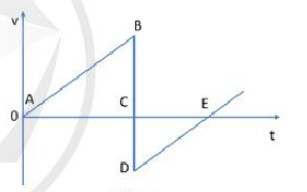
\includegraphics[scale=1]{figs/G10Y25B7-3}
	\end{center}
	
	\begin{enumerate}[label=\alph*)]
		\item Tại sao độ dốc của đoạn thẳng AB lại giống độ dốc của đoạn thẳng DE?
		\item Diện tích tam giác ABC biểu thị đại lượng nào?
	\end{enumerate}
	\loigiai{	
		\begin{enumerate}[label=\alph*)]
			\item Trong quá trình rơi xuống và bật ngược trở lại, quả bóng chuyển động với gia tốc bằng gia tốc rơi tự do. Do đó, độ dốc của đường thẳng AB và DE có giá trị bằng nhau và bằng gia tốc rơi tự do.
			
			\item Diện tích tam giác ABC biểu diễn quãng đường dịch chuyển của quả bóng từ A đến B.
			
		\end{enumerate}
	}
\end{ex}
\Closesolutionfile{ans}
	